% chapters/chapter1/1_1_intro.tex
% !TeX root=../../main.tex

\section{مقدمه}

جرثقیل‌های سقفی شریان‌های اصلی انتقال مواد در سایت‌های صنعتی و محیط‌های لجستیکی به شمار می‌آیند (شکل \ref{fig:real_crane}). چالش بنیادین در طراحی سیستم‌های هدایت این تجهیزات، ماهیت زیرفعال (\lr{Underactuated}) و دینامیک نوسانی آن‌هاست. انتقال سریع کالسکه و اعمال شتاب در ابتدا و انتهای مسیر، ناگزیر به تحریک دینامیک ارتعاشی مهارنشده در بار آویخته می‌انجامد. این نوسانات علاوه بر کاهش دقت موقعیت‌یابی و افزایش زمان چرخه کاری، مخاطرات ایمنی جدی به همراه دارند. فراتر از مسئله ایمنی، نوسانات پاندول و اعمال شوک‌های شتاب، موجب ایجاد نیروهای دینامیکی متناوب در سازه می‌شوند. مهار این نیروها برای پیشگیری از پدیده خستگی (\lr{Fatigue}) در سازه، کاهش استهلاک مفاصل مکانیکی و در نهایت افزایش طول عمر تجهیزات، از منظر مهندسی مکانیک اهمیتی حیاتی دارد. بر این اساس، ارزیابی کمی تأثیر معماری‌های کنترلی بر پروفایل نیروهای وارد بر سازه، یکی از اهداف محوری این پژوهش است.

\begin{figure}[htbp]
    \centering
    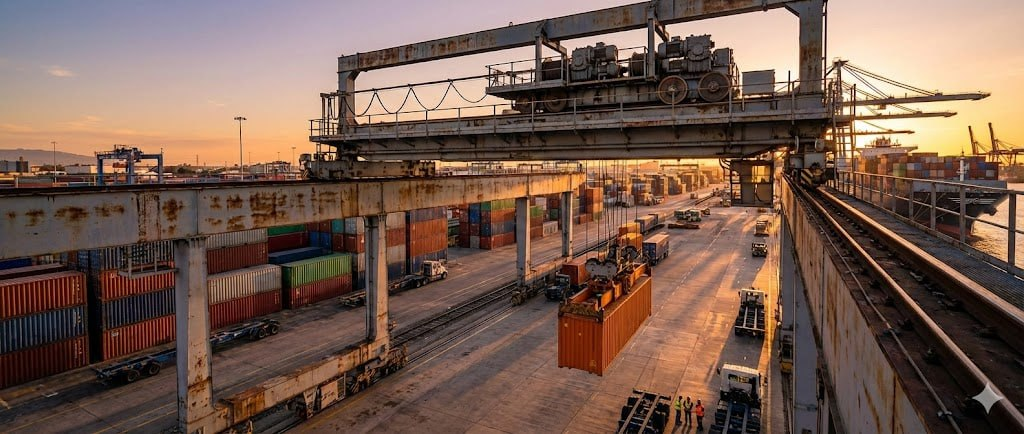
\includegraphics[width=0.8\textwidth]{images/0_System_Modeling/real_image.jpg}
    \caption{نمای کلی از عملکرد جرثقیل‌های سقفی در سایت‌های صنعتی و اهمیت مهار نوسانات در حین انتقال بار.}
    \label{fig:real_crane}
\end{figure}

مهار هم‌زمان نوسان‌ها در طول مسیر و حذف نوسان پسماند (\lr{Residual Sway}) در زمان توقف، مسئله‌ای است که روش‌های کنترل کلاسیک در مواجهه با آن دچار محدودیت هستند. برای حل این چالش، پژوهش حاضر از یک استراتژی یکپارچه بهره می‌برد. در این روش، عملگر وینچ (مکانیزم تغییر طول کابل) همگام با نیروی محرک کالسکه، نقش یک سیستم میرایی فعال (\lr{Active Damping}) را ایفا می‌کند. این معماری با تنظیم هماهنگی فاز (\lr{Phase Matching}) بین سرعت کابل و نوسان بار، نیروهای کوپل‌شده سینماتیکی نظیر کوریولیس را برای استهلاک پیوسته انرژی به کار می‌گیرد؛ در نتیجه، استراتژی کنترل‌کننده صرفاً به کاهش فرکانس طبیعی تقلیل نمی‌یابد. شماتیک مکانیکی این جرثقیل و مفصل متغیر آن در شکل \ref{fig:schematic_crane} ترسیم شده است.

\begin{figure}[htbp]
    \centering
    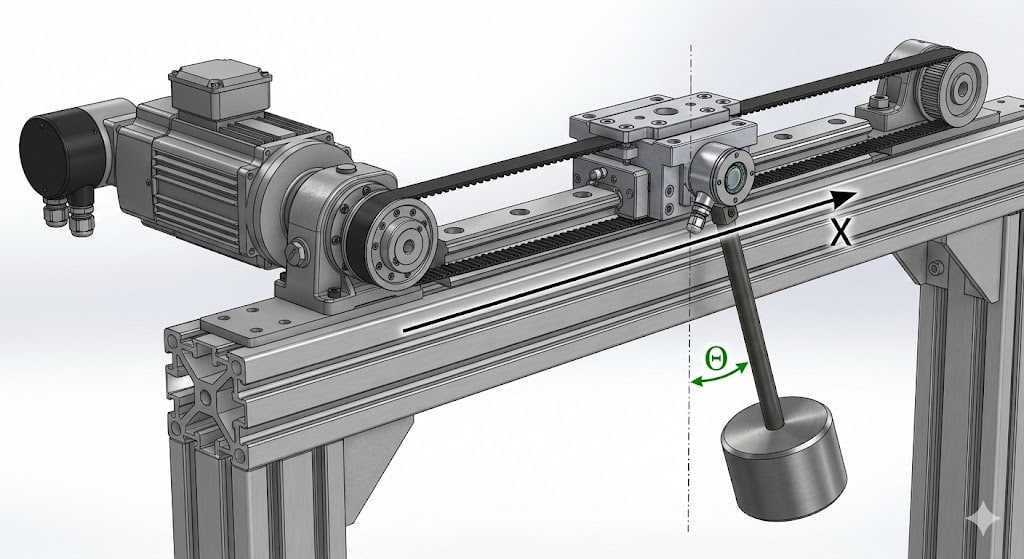
\includegraphics[width=0.8\textwidth]{images/0_System_Modeling/schematic_image.jpg}
    \caption{شماتیک طراحی و پروتوتایپ آزمایشگاهی سیستم جرثقیل سقفی با مفصل کشویی متغیر (تغییر طول کابل).}
    \label{fig:schematic_crane}
\end{figure}

در این راستا، فصل حاضر ساختار دینامیکی جرثقیل سقفی را تدوین می‌کند. در گام نخست، مدل‌سازی سینماتیکی و سینتیکی با رویکرد تحلیلی اویلر-لاگرانژ انجام می‌گیرد و معادلات حرکت سیستم استخراج می‌شوند. پس از آن، برای ایجاد یک معیار ارزیابی پایه (\lr{Benchmark})، مدل فضای حالت حول وضعیت تعادل آویزان خطی‌سازی شده و یک کنترل‌کننده فیدبک حالت بهینه از نوع تنظیم‌گر خطی درجه دوم (\lr{LQR}) طراحی می‌شود.

تحلیل‌های ریاضی و شبیه‌سازی‌ها در این فصل نشان می‌دهند که در تقریب خطی بسط تیلور پیرامون نقطه کار، عملگر تغییر طول کابل اثرگذاری محلی خود را از دست می‌دهد. همچنین، اعمال مستقیم خطاهای موقعیت بزرگ در قالب ورودی پله به کنترل‌کننده خطی، به دلیل نقض فرضیات زوایای کوچک و اشباع شدید نیروی محرک، به ناپایداری دینامیکی و چرخش کامل آونگ می‌انجامد. این محدودیت‌های ساختاری، ضرورت عبور از تئوری کنترل کلاسیک و استقرار یک معماری یکپارچه مبتنی بر برنامه‌ریز مسیر سینماتیکی و کنترل پیش‌بین مدل غیرخطی (\lr{NMPC}) را برای فصول آتی توجیه می‌کند؛ معماری پیشرفته‌ای که با اشراف بر دینامیک غیرخطی، می‌تواند از تمامی عملگرها به‌صورت هم‌زمان و در حضور قیود فیزیکی برای هدایت سیستم و سرکوب نوسانات بهره ببرد.